%%% License: Creative Commons Attribution Share Alike 4.0 (see https://creativecommons.org/licenses/by-sa/4.0/)
%%% Slides are based heavily on earlier versions of this course taught by Jesper Rudiger.

\documentclass[english,10pt
%,handout
,aspectratio=169
]{beamer}
%%% License: Creative Commons Attribution Share Alike 4.0 (see https://creativecommons.org/licenses/by-sa/4.0/)
%%% Slides are based heavily on earlier versions of this course taught by Jesper Rudiger and Peter Norman Sorensen.

\DeclareGraphicsExtensions{.eps, .pdf,.png,.jpg,.mps,}
\usetheme{reMedian}
\usepackage{parskip}
\makeatother

\renewcommand{\baselinestretch}{1.1} 

\usepackage{amsmath, amssymb, amsfonts, amsthm}
\usepackage{enumerate}
\usepackage{hyperref}
\usepackage{url}
\usepackage{bbm}
\usepackage{color}

\usepackage{tikz}
\usepackage{tikzscale}
\newcommand*\circled[1]{\tikz[baseline=(char.base)]{
		\node[shape=circle,draw, inner sep=-20pt] (char) {#1};}}
\usetikzlibrary{automata,positioning}
\usetikzlibrary{decorations.pathreplacing}
\usepackage{pgfplots}
\usepgfplotslibrary{fillbetween}
\usepackage{graphicx}

\usepackage{setspace}
%\thinmuskip=1mu
%\medmuskip=1mu 
%\thickmuskip=1mu 


\usecolortheme{default}
\usepackage{verbatim}
\usepackage[normalem]{ulem}

\usepackage{apptools}
\AtAppendix{
	\setbeamertemplate{frame numbering}[none]
}
\usepackage{natbib}



\title{Financial Markets Microstructure \\ Lecture 15}

\subtitle{Auction Models}

\author{Egor Starkov}

\date{K{\o}benhavns Unversitet \\
	Spring 2020}


\begin{document}
	\AtBeginSection[]{
		\frame<beamer>{
			\frametitle{This lecture:}
			\tableofcontents[currentsection,currentsubsection]
	}}
	\frame[plain]{\titlepage}



\begin{frame}{Previously on FMM}
	\begin{itemize}
		%\item \textbf{Bubbles}
		\item \textbf{Smith \& S{\o}rensen / Bikchandhani \& Sharma}:
		\begin{itemize}
			\item Verious models of \structure{herding}
			\item If public information is informative enough, it can lead traders to ignore their private signals
			\item But public information need not always be correct
		\end{itemize}
		\item \textbf{Abreu \& Brunnermeier}:
		\begin{itemize}
			\item Theory of \structure{bubbles}
			\item No common knowledge $\Rightarrow$ no one sure when the bubble will burst even if everyone informed of the mispricing
			\item Incentives to ride the bubble can outweigh the risk
		\end{itemize}
	\end{itemize}
\end{frame}	


\begin{frame}{Today}
	\begin{itemize}
		\item We have talked extensively about \alert{dealer markets} and mentioned a couple of \alert{continuous-auction} models
		\item Have not talked much about \structure{call auctions} (except Kyle model, which was still dealer-centric)
		\item Hence today -- \textbf{Auction models}
		\begin{itemize}
			\item Very prominent in Econ in general
			\item Not too specific to FinMarkets
			\item Will do a quick intro via the most relevant model(s?)
		\end{itemize}
	\end{itemize}
\end{frame}


\begin{frame}{Introduction to Auctions}
	\begin{itemize}
		\item Auction theory -- one of the big successes of game theory in the 80s/90s
		\item Active field of research to this day
		\item Widely used:
		\begin{itemize}
			\item Google ads
			\item Spectrum auctions
			\item Privatisation?
			\item Financial markets?
		\end{itemize}
		\item Main point: capturing imperfect competition in the presence of a finite number of agents in the market
	\end{itemize}
\end{frame}


\begin{frame}
	\center
	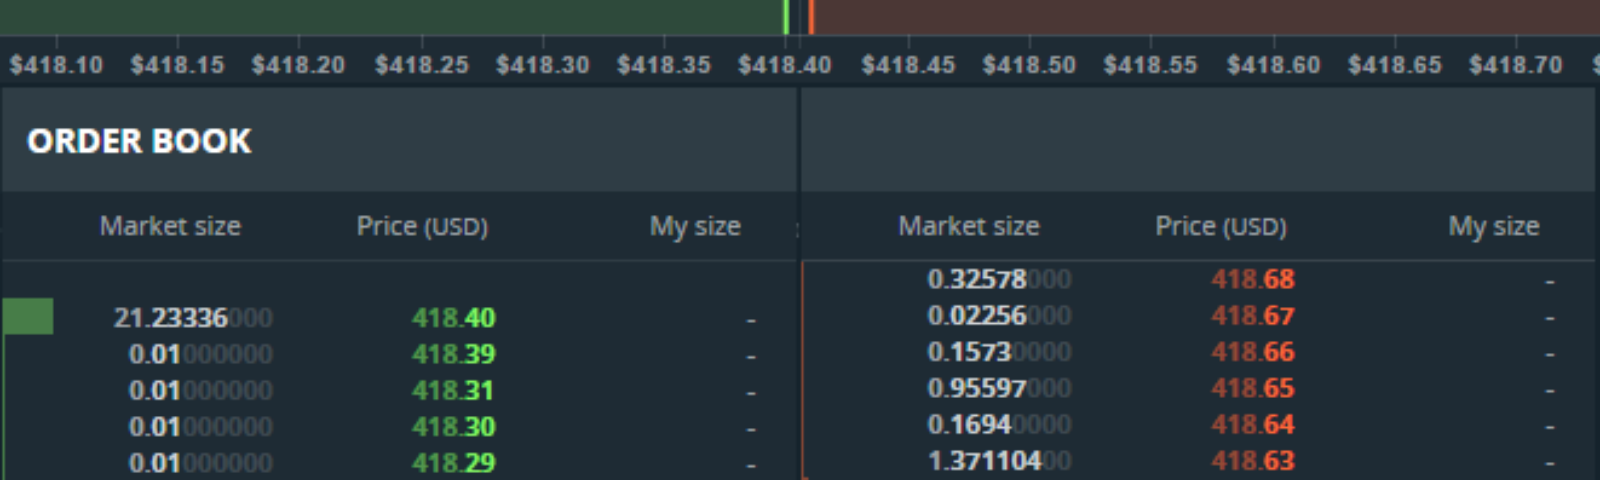
\includegraphics[width=\linewidth]{pics/LOB}
\end{frame}


\begin{frame}{Models}
	\begin{itemize}
		\item There is huge variety of auction types you can consider (and most are somewhat tractable):
		\begin{itemize}
			\item plethora of \structure{formats} (open/sealed-bid, first-/second-/Xth-price, winner-pay or all-pay)
			\item \structure{symmetric} or \structure{asymmetric} information;
			\item \structure{private} or \structure{common} valuations;
			\item \structure{single-} or \structure{multi-} unit;
			\item \structure{single-sided} or \structure{double} auctions;
			\item known or unknown \structure{number of bidders};
			\item \structure{symmetric} or \structure{asymmetric} bidders.
		\end{itemize}
		\pause
		\item Will look at some of these
		\item Will follow parts of \cite{krishna_auction_2009}, see that book for more on auction theory
	\end{itemize}
\end{frame}


\section{Private-value First-price Auction}

\begin{frame}{Private-value First-price Auction: Setup}
	\begin{itemize}
		\item One \structure{item} for sale
		\item $N$ \structure{bidders} $i \in \{1,...,N\}$
		\begin{itemize}
			\item Everyone has a private valuation $x_i \in [0,\bar{x}]$ for the item, i.i.d.
		\end{itemize}
		\item Everyone simultaneously submits bid $b_i$
		\item Highest bid wins, pays $b_i$, rest pay nothing
		\item All agents maximize expected profit
		\[ 
			\Pi(b_i,x_i) = \left( x_i - b_i \right) \cdot \mathbb{P} \left( b_i \geq \max_{j\neq i} b_j \right) 
		\]
	\end{itemize}
\end{frame}


\begin{frame}{PV FPA: Equilibrium}
	\begin{itemize}
		\item Trade-off: bidding higher wins more often, but gives lower payoff
		\item Look for symmetric equilibrium:
		\begin{itemize}
			\item Suppose all $j\neq i$ use some bidding strategy $\beta(x)$ (strictly increasing and differentiable)
			\item Find optimal bid $b_i(x_i)$.
			\item In symm eqm must have $b_i(x_i) = \beta(x_i)$.
		\end{itemize}
		\item Any bid $b_i > \beta(\bar{x})$ is strictly dominated by $b_i = \beta(\bar{x})$.
		\item If $x_i=0$ then dominant to bid $b_i=0$ $\Rightarrow \beta(0)=0$.
	\end{itemize}
\end{frame}


\begin{frame}{PV FPA: Solving for eqm}
	\begin{itemize}
		\item Let $G(\cdot)$ be cdf of $y_1 = \max_{j\neq i} x_j$, $g(\cdot)$ is pdf
		\begin{itemize}
			\item highest valuation among all opponents
		\end{itemize}
		\item Bid $b$ must maximize expected profit:
		\[ \Pi(b,x) = (x-b) \cdot G \left( \beta^{-1}(b) \right) \]
		\item FOC wrt $b$:
		\[ \frac{g\left( \beta^{-1}(b) \right)}{\beta' \left( \beta^{-1}(b) \right)} (x-b) - G\left( \beta^{-1}(b) \right) = 0 \]
		\item This condition yields optimal $b$ in terms of $x$ and $\beta(\cdot)$.
	\end{itemize}
\end{frame}


\begin{frame}{PV FPA: Solving for eqm}
	\begin{itemize}
		\item As mentioned before, in eqm must be $b = \beta(x)$. Plug that into the FOC to get the differential eqn:
		\[ G(x) \beta'(x) + g(x) \beta(x) = xg(x) \]
		\item Can solve DE to get the \structure{eqm strategy}
		\[ \beta(x) = \frac{1}{G(x)} \int_0^x yg(y) dy = \mathbb{E}[y_1 | y_1<x] \]
		\begin{itemize}
			\item Bid the expected value of the strongest opponent -- conditional on winning the auction
		\end{itemize}
	\end{itemize}
\end{frame}


\begin{frame}{PV FPA: Example}
	\begin{itemize}
		\item Suppose $x_i \sim U[0,1]$
		\item Then for $x_i\in [0,1]$: $F(x) = x$ and $G(x) = \pause F^{N-1}(x)= x^{N-1}$
		\item Computing the equilibrium strategy yields
		\[ \beta(x) = \frac{N-1}{N} x \]
	\end{itemize}
\end{frame}


\begin{frame}{PV FPA: Conclusions}
	\[ \beta(x) = \mathbb{E}[y_1 | y_1<x] \]
	\begin{itemize}
		\item \structure{bids} $b$ are ``\structure{shaded}'' compared to valuation (i.e., $b < x$)
		\item degree of shading depends on $N$ (large shading is costlier with more opponents)
		\item bidders not perfectly competitive $\rightarrow$ get positive profits
		\begin{itemize}
			\item partly due to asymmetric information (but no adverse selection)
		\end{itemize}
		\item beliefs about the distribution of others' valuations $x_j$ matter a lot for this derivation
	\end{itemize}
\end{frame}


\begin{frame}{Interlude}
	\begin{itemize}
		\item This was one of the most standard models -- but the approach is pretty universal
		\item Many dimensions in which it is not a perfect fit for our purposes:
		\item (1) \alert{Bids are simultaneous and unobservable}
		\begin{itemize}
			\item There are some more fitting formats we can look at:
			\item \structure{English auction} (ascending-price) is payoff-equivalent (in IPV setting)
			\item \structure{Dutch auction} (descending-price) is payoff- and strategy-equivalent
		\end{itemize}
		\item (2) \alert{Private values} -- look at common-value model now
		\item (3) \alert{Single-unit, single-side} 
		\begin{itemize}
			\item \structure{multi-unit auctions} are not much different if profit linear in quantity -- with $k$ items just need to win against $k$th-highest bid of the opponents (rather than the top)
			\item \structure{double auctions} -- later today
		\end{itemize}
	\end{itemize}
\end{frame}




\section{Common-value First-price Auction}

\begin{frame}{Common-value First-price Auction: Setup}
	%Ch 6.4 of Krishna
	\begin{itemize}
		\item One \structure{item} of \alert{value $v$} for sale
		\item $N$ \structure{bidders} $i \in \{1,...,N\}$
		\begin{itemize}
			\item No one knows $v$ for sure
			\item Everyone gets a private signal $x_i = v+\epsilon_i$ with $\epsilon_i$ i.i.d., $\mathbb{E}[\epsilon_i]=0$
			\item Suppose $x_i \in [0,\bar{x}]$
		\end{itemize}
		\item Everyone simultaneously submits bid $b_i$
		\item Highest bid wins, pays $b_i$, rest pay nothing
		\item All agents maximize expected profit
		\[ 
			\Pi(b_i,x_i) = \mathbb{E} \left[ v - b_i | x_i, b_i \geq \max_{j\neq i} b_j \right] \cdot \mathbb{P} \left( b_i \geq \max_{j\neq i} b_j \right) 
		\]
	\end{itemize}
	%mention winner's curse?
\end{frame}


\begin{frame}{CV vs PV}
	\begin{itemize}
		\item What changed relative to private-value case?
		\item \structure{Valuation} is now not $x_i$, but $\mathbb{E} \left[ v | x_i, \alert<2>{b_i \geq \max_{j\neq i} b_j} \right]$
		\pause
		\begin{itemize}
			\item Suppose equilibrium bidding strategy $\beta(x)$ is monotone in signal $x$
			\item If you won -- everyone else bid less -- everyone else had worse info
			\item \alert{Winner's curse}: $\mathbb{E} \left[ v | x_i, b_i \geq \max_{j\neq i} b_j \right] < \mathbb{E} \left[ v | x_i \right]$
		\end{itemize}
	\end{itemize}
\end{frame}


\begin{frame}{CV FPA: Solving the model}
	\begin{itemize}
		\item Suppose all agents $j\neq i$ follow the same bidding strategy $\beta(x)$
		\begin{itemize}
			\item increasing and differentiable
		\end{itemize}
		%\item Will derive the optimal strategy $\beta_i(x_i)$ for $i$ -- in eqm must have $\beta = \beta_i$
		\item Let $G(\cdot|x)$ be cdf of $y_1 = \max_{j\neq i} x_j$ conditional on $x_i=x$, $g(\cdot|x)$ is pdf
		\item Let $v(x,y) = \mathbb{E} \left[ v | x_i=x, y_1=y \right]$
		\item Suppose $i$ has signal $x_i=x$ and bids $b_i = \beta(z)$ for some $z$
		\begin{itemize}
			\item then $i$ wins whenever $y_1 < z$
			\item (in eqm must be optimal to bid s.t. $z=x$)
		\end{itemize}
		\begin{align*}
			\Pi(\beta(z),x) &= \int_0^z \left[ v(x,y) - \beta(z) \right] g(y|x) dy
			\\
			&= \int_0^z v(x,y) g(y|x) dy - \beta(z) G(z|x)
		\end{align*}
	\end{itemize}
\end{frame}


\begin{frame}{CV FPA: Solving the model}
	\[ \Pi(\beta(z),x) = \int_0^z v(x,y) g(y|x) dy - \beta(z) G(z|x) \]
	Take FOC w.r.t $z$:
	\[ 
		\left[ v(x,z) - \beta(z) \right] g(z|x) - \beta'(z)G(z|x) = 0
	\]
	As we said, in eqm must be $z=x$. Plugging that into the FOC we get the differential eqn for the eqm strategy:
	\[ \beta'(x) = \left[ v(x,x) - \beta(x) \right] \frac{g(x|x)}{G(x|x)} \]
	Boundary condition: $\beta(0)=0$. Solve DE to obtain the closed-form expression for \structure{eqm strategies}:
	\[ \beta(x) = \int_0^x v(y,y) dL(y|x) \]
	where $L(y|x) = \exp \left\{ -\int_x^y \frac{g(t|t)}{G(t|t)} dt \right\}$.
\end{frame}


\begin{frame}{CV FPA: Example}
	\begin{itemize}
		\item Let $N=2$, each player observes $x_i = s_i + t$, where $s_1,s_2,t \sim \text{i.i.d.}U[0,1]$
		\item Asset value $v = \frac{1}{2} (x_1 + x_2)$
		\begin{itemize}
			\item (not the case that $\mathbb{E}[\epsilon_i]=0$, but still the common-value setting)
		\end{itemize}
		\item If you solve for eqm, get $\beta(x) = \frac{2}{3} x$
	\end{itemize}
\end{frame}


\begin{frame}{CV FPA: Conclusions}
	\[ \beta(x) = \int_0^x v(y,y) dL(y|x) \]
	\begin{itemize}
		\item Two sources of bid shading: one is same as in PV case, another due to winner's curse
		\item Integral for same reasons as before
		\item Winner's curse: integrating over \alert{$v(y,y)$} 
		\begin{itemize}
			\item Accounts for some adverse selection -- conditions on $y_2 < y$
			\item Not $v(x,y)$ -- ignoring own signal $x$, and $v(y,y)<v(x,y)$ for $y<x$.
			\item Clearer if you look at Second-Price Auctions.
		\end{itemize}
	\end{itemize}
\end{frame}


\section{Second-price Auctions}

\begin{frame}{Second-price Auctions}
	\begin{itemize}
		\item Consider two settings, which are as above (private- \& common-value), but now the winner pays \alert{second-highest price}
		\item With private valuations the expected profit is then
		\[ 
			\Pi(b_i,x_i) = \left( x_i - \alert{\max_{j\neq i} b_j} \right) \cdot \mathbb{P} \left( b_i \geq \max_{j\neq i} b_j \right) 
		\]
		\item In the common-value setting:
		\[ 
			\Pi(b_i,x_i) = \mathbb{E} \left[ v - \alert{\max_{j\neq i} b_j} \mid x_i, b_i \geq \max_{j\neq i} b_j \right] \cdot \mathbb{P} \left( b_i \geq \max_{j\neq i} b_j \right) 
		\]
	\end{itemize}
\end{frame}


\begin{frame}{SPA: Equilibria}
	\begin{block}{}
		In PV-SPA, $\beta(x)=x$ is a weakly dominant strategy for all players.
	\end{block}
	\pause
	\begin{block}{}
		In CV-SPA, $\beta(x)=v(x,x)$ constitutes a symmetric equilibrium.
	\end{block}
	Note that ``own value'' is $v(x,x)$, not $\mathbb{E} \left[v(x,y)\right]$, not $\mathbb{E} \left[v(x,y) | y \leq x \right]$. 
	\begin{itemize}
		\item Meaning bids are higher than one would naively expect
		\item Adverse selection baked into $v(x,y)$ via conditioning on $y_2 < y$
	\end{itemize}
\end{frame}


\section{Double Auctions}

\begin{frame}{Double Auction}
	\begin{itemize}
		\item Double Auction (\cite{chatterjee_bargaining_1983}) is pretty similar to FPA. To illustrate, look at PV version:
		\item One \structure{item} for sale
		\item Two agents: seller and buyer (bilateral monopoly), $i \in \{S,B\}$
		\begin{itemize}
			\item Both have private valuations $x_i \in [0,\bar{x}]$ for the item, independent
		\end{itemize}
		\item Simultaneously submit bids $b_i$
		\item If $b_B > b_S$, trade happens at price $b_B$ (for example)
		\item All agents maximize expected profits:
		\begin{align*}
			\Pi_B(b_B,x_B) = \left( x_B - b_B \right) \cdot \mathbb{P} \left( b_B \geq b_S \right) 
			\\
			\Pi_S(b_S,x_S) = \left( b_B - x_S \right) \cdot \mathbb{P} \left( b_B \geq b_S \right) 
		\end{align*}
	\end{itemize}
\end{frame}


\begin{frame}{Double Auction: Solution}
	\begin{itemize}
		\item Note that this is a PV-SPA for the seller and PV-FPA for the buyer
		\item Hence seller bids $\beta_S(x_S) = x_S$ (weakly dominant);
		\item Buyer solves
		\[ \max_{b_B} \left( x_B - b_B \right) \cdot F_S(b_B) \]
		\item E.g., if $x_i \sim \text{i.i.d.} U[0,1]$ then $\beta_B(x_B) = x_B/2$.
	\end{itemize}
\end{frame}


\begin{frame}{Double Auction: Inefficiency}
	\begin{itemize}
		\item Note that DA outcome is \alert{inefficient}, unlike in one-sided auctions:
		\begin{itemize}
			\item Trade happens in equilibrium iff $x_B/2 > x_S$
			\item Efficient to trade iff $x_B > x_S$
		\end{itemize}
		\item Myerson-Satterthwaite theorem: there is no trading protocol that yields the efficient outcome in this problem (and does not run a deficit).
	\end{itemize}
\end{frame}



\begin{frame}{Conclusion}
	\begin{enumerate}
		\item Auctions are fun
		\item Two sources of bid shading: market power and winner's curse
		\item Second-price auctions are simple and robust
		\item Efficient outcome is difficult to obtain in bilateral trade setting
	\end{enumerate}
\end{frame}



\appendix
\begin{frame}[allowframebreaks]{References}
	\bibliography{../teaching}
	\bibliographystyle{abbrvnat}
\end{frame}

\end{document} 